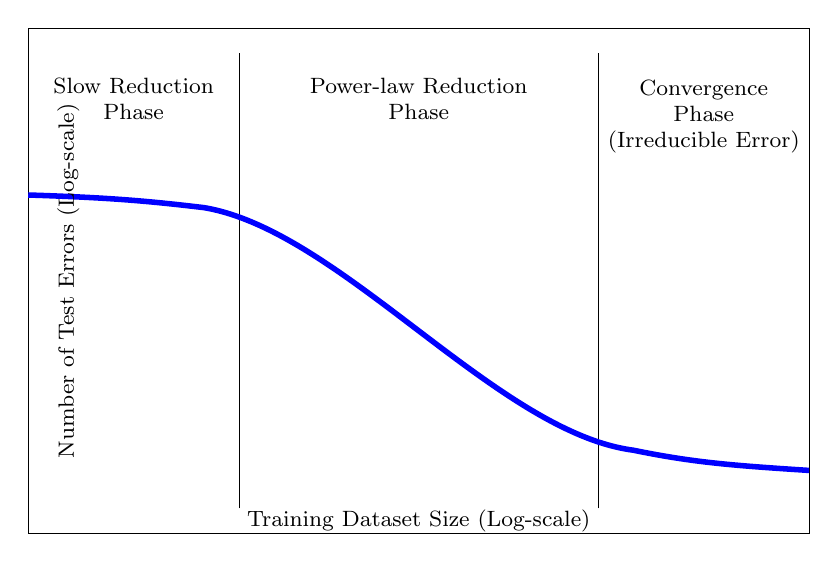
\begin{tikzpicture}

\def\upline{13.5}
\def\downline{2.5}
\def\upcenpos{17.2}

\begin{scope}
\begin{axis}[
width=11.5cm, height=8cm,
xlabel={Training Dataset Size (Log-scale)},
ylabel={Number of Test Errors (Log-scale)},
xlabel style={align=center,yshift=1.2em,font=\footnotesize},
ylabel style={align=center,yshift=-2.2em,font=\footnotesize},
xticklabel style={fill=white,opacity=0},
yticklabel style={fill=white,opacity=0},
x tick style={fill=white,opacity=0},
y tick style={fill=white,opacity=0},
xtick=\empty,
ytick=\empty,
legend pos=outer north east,
xmin=0,
xmax=100,
ymin=0,
ymax=20]


\addplot [sharp plot] coordinates{(27,1) (27,19)};
\addplot [sharp plot] coordinates{(73,1) (73,19)};

{\footnotesize
\node[anchor=center,align=center,font=\footnotesize] (t1) at (axis cs:13.5,\upcenpos) {Slow Reduction\\ Phase};
\node[anchor=center,align=center,font=\footnotesize] (t2) at (axis cs:50,\upcenpos){Power-law Reduction\\ Phase};
\node[anchor=center, align=center,font=\footnotesize] (t3) at (axis cs:86.5,\upcenpos - 0.7) {Convergence \\ Phase \\ (Irreducible Error)};


\draw[-,line width=2pt,blue] (axis cs:0,\upline-0.1) .. controls ([xshift=0em,yshift=0em]axis cs:10,\upline-0.199) and ([xshift=0em,yshift=0em]axis cs:15,\upline-0.32275) .. (axis cs:22.5,\upline-0.6) .. controls ([xshift=0em,yshift=0em]axis cs:40,12) and ([xshift=0em,yshift=0em]axis cs:60,4) .. (axis cs:77.5,\downline+0.8) .. controls ([xshift=0em,yshift=0em]axis cs:85,\downline+0.32275) and ([xshift=0em,yshift=0em]axis cs:90,\downline+0.199) .. (axis cs:100,\downline);
}
\end{axis}
\end{scope}
\end{tikzpicture}
